% =====================================================================
% DRAFT v1 (11.11.2026) -- crossing neighborhoods for the PFSP:
% Dynasearch -> Motzkin -> single crossings -> involutions.
% Target: GECCO 2027 (deadline unconfirmed); double-blind.
% Layout: plain article class for drafting; switch to the official
% template once the CFP is out.
% Protocol = identical to the previous papers of this line (same ILS,
% same constants, same budgets, same accelerator); the neighborhood
% family is the only factor of the main study. The safeguard (safe rule)
% is a separate variant with its own section and table (decision of
% 11.11.2026: it changes the selection rule, not the neighborhood).
% Tables marked PILOT hold pilot data (4 instances x 3 seeds, cloud
% timings, 50x10 seeds not confirmed as ta041-ta044); they are
% placeholders; numbers from the Mac rerun. The pilot used no block filter (all pairs). Table "main"
% is a skeleton.
% Bibliography: every entry must be verified in Crossref before use.
% =====================================================================
\documentclass[10pt,twocolumn]{article}
\usepackage[margin=0.75in]{geometry}
\usepackage[T1]{fontenc}
\usepackage{amsmath,amssymb,amsthm}
\usepackage{booktabs}
\usepackage{multirow}
\usepackage{xcolor}
\usepackage{tikz}
\usepackage[hidelinks]{hyperref}

\newtheorem{proposition}{Proposition}
\newtheorem{lemma}{Lemma}
\newtheorem{definition}{Definition}
\newcommand{\todo}[1]{\textcolor{red}{[TODO: #1]}}
\newcommand{\N}{\mathcal{N}}
\newcommand{\Pa}{\mathcal{P}}
\newcommand{\ncr}{\operatorname{cr}}

\title{Should Swaps Cross? Compound-Swap Neighborhoods from Motzkin\\
to Involutions for the Permutation Flow Shop}
\author{Anonymous submission}
\date{}

\begin{document}
\maketitle

\begin{abstract}
A compound move for the permutation flow shop applies several endpoint
swaps at once and is chosen by an exact algorithm that minimizes the sum
of the individual makespan changes. Dynasearch allows only swaps on
disjoint intervals, and the Motzkin neighborhood also allows nested
ones. We complete this axis. The family $\N_c$ admits at most $c$
crossing pairs of swaps, $\Pa_1$ lets every swap cross at most one
other, and the largest member is the set of all involutions. We count
these neighborhoods with a continued fraction and show that a bounded
number of crossings multiplies the Motzkin number only by a polynomial
factor, $|\N_c|\sim M_n (n/3)^c/c!$. The best move is found exactly by
an interval dynamic program for $c=0$, by a dynamic program over
two-arc cores for $c=1$ and $\Pa_1$, and by maximum-weight matching for
involutions. All families share the candidate swaps and their deltas, so
the selection adds little to the $O(mn^3)$ cost of the deltas. The limit
is additivity. Two improving swaps on disjoint intervals realize a
larger share of their predicted joint gain than two nested or crossing
swaps. Under additive selection the quality of iterated local search
should therefore fall along the axis, and disjoint swaps should be the
best choice. \todo{headline result of the campaign}
\end{abstract}

% ---------------------------------------------------------------------
\section{Introduction}

The permutation flow shop scheduling problem with the makespan
criterion, $F|prmu|C_{\max}$, is NP-hard for $m\geq 3$
machines~\cite{garey1976} and is a standard testbed for local
search~\cite{taillard1993,ruiz2007}. Dynasearch~\cite{congram2002}
showed that an exponential set of independent pairwise interchanges can
be searched exactly by dynamic programming, which makes a compound move
the unit of search within very large-scale neighborhood
search~\cite{ahuja2002}. For the flow shop, two compound neighborhoods
of endpoint swaps are in use. Dynasearch combines swaps whose intervals
are pairwise disjoint. The Motzkin neighborhood~\cite{motzkin_own} also
admits nested swaps and is counted by the Motzkin numbers.

Both neighborhoods forbid one configuration: two swaps $(a,b)$ and
$(c,d)$ with $a<c<b<d$, which cross when drawn as arcs over the
permutation. Nothing in the move itself requires this. Any set of swaps
with pairwise distinct endpoints is an involution and defines a valid
neighbor, and the best involution under an additive objective is a
maximum-weight matching, which is polynomial. The ban on crossings
exists because the interval dynamic program cannot express them. This
paper asks whether the ban costs anything: \emph{should swaps in a
compound move be allowed to cross?}

We answer with a family of neighborhoods ordered by how much two swaps
may overlap. It starts at Dynasearch, passes through Motzkin and through
moves with a bounded number of crossings, and ends at all involutions.
The whole family uses one set of candidate swaps and one set of deltas,
so its members differ only in which subsets of candidates they may
select. This isolates the effect of overlap from the effect of cost. We
keep the metaheuristic, its parameters and the experimental protocol of
the earlier studies~\cite{motzkin_own,windowed_own} unchanged, so every
new number can be read against the published ones.

The paper makes four contributions. First, it defines the crossing
families $\N_c$ and $\Pa_r$ and counts them. A continued fraction gives
the exact sizes, and a Poisson-type lemma shows that a constant number
of crossings leaves the growth rate at $3^n$, whereas all involutions
grow faster than any exponential. Second, it gives exact selection
algorithms for every level of the axis and shows that they are cheap
next to the deltas they consume. Third, it measures how additivity
depends on the geometry of a pair of swaps: disjoint, nested or
crossing. This measurement explains why larger neighborhoods of this
kind predict more and deliver less. Fourth, it evaluates the families on
the Taillard benchmark under the selection rule of the earlier studies
and reports what compound moves add over the best single swap. A
separate variant that checks the real makespan of the selected move
once shows how much of the loss this check removes.
\todo{optional fifth: QUBO density versus neighborhood size on quantum
hardware, Section~\ref{sec:quantum}}

% ---------------------------------------------------------------------
\section{Background}

\paragraph{Compound moves in scheduling.} Dynasearch was introduced for
single-machine total weighted tardiness~\cite{congram2002}; later work
made its search faster~\cite{ergun2006} and added
insertions~\cite{grosso2004}. Bo\.zejko and Wodecki analyzed swap
multimoves for the flow shop~\cite{bozejko2007}. The Fibonacci
neighborhood combines disjoint adjacent
swaps~\cite{fibonacci_own,bozejko2026sr}, and the Motzkin neighborhood
combines noncrossing swaps~\cite{motzkin_own}. In total weighted
tardiness the cost changes of independent swaps add up and the dynamic
program is exact. In the flow shop they do not, so every one of these
neighborhoods optimizes a surrogate.

\paragraph{Neighborhoods searched by matching.} Sarvanov and
Doroshko~\cite{sarvanov1981} and Gutin~\cite{gutin1999} search
factorial-size neighborhoods of the travelling salesman problem by an
assignment problem, and Deineko and Woeginger~\cite{deineko2000} survey
exponential neighborhoods for the travelling salesman and quadratic
assignment problems. The involution neighborhood belongs to this
tradition. What has not been studied is the axis between the interval
program and the matching, and whether moving along it helps.

\paragraph{RNA secondary structure.} The same axis exists in RNA
folding, where base pairs are arcs over a sequence. Nussinov's
algorithm~\cite{nussinov1978} is the noncrossing interval program.
Pseudoknots are crossings: Rivas and Eddy~\cite{rivas1999} and
Akutsu~\cite{akutsu2000} give dynamic programs for restricted classes,
general pseudoknots are NP-hard in energy models~\cite{lyngso2000}, and
Tabaska et al.~\cite{tabaska1998} obtain arbitrary pseudoknots from a
maximum-weight matching when the score is additive. Our level $c=0$
corresponds to Nussinov's algorithm, $c=1$ to a simple pseudoknot, and
involutions to the matching approach.

\paragraph{Crossings in matchings.} The distribution of crossings in
matchings and involutions is classical~\cite{touchard1952,riordan1975}
and has a continued-fraction form~\cite{flajolet1980}. Crossings and
nestings are equidistributed~\cite{kasraoui2006}, and $k$-noncrossing
matchings were counted by Chen et al.~\cite{chen2007}. We use these
results to size the neighborhoods.

% ---------------------------------------------------------------------
\section{The Crossing Family}\label{sec:family}

$n$ jobs are processed on machines $1,\dots,m$ in the order
$\pi=(\pi(1),\dots,\pi(n))$, and $p_{r,j}$ is the processing time of job
$j$ on machine $r$. Completion times satisfy
$C_{r,t}=\max(C_{r-1,t},C_{r,t-1})+p_{r,\pi(t)}$ and
$C_{\max}(\pi)=C_{m,n}$.

\begin{definition}
An \emph{elementary move} $s(i,j)$, $i<j$, exchanges $\pi(i)$ and
$\pi(j)$ and leaves the jobs between them in place. A \emph{compound
move} is a set $\sigma$ of elementary moves with pairwise distinct
endpoints, that is, an involution of the positions; the neighbor is
$\pi\circ\sigma$. Two swaps $(a,b)$ and $(c,d)$ with $a<c$ are
\emph{disjoint} if $b<c$, \emph{nested} if $d<b$, and \emph{crossing} if
$c<b<d$. $\ncr(\sigma)$ is the number of crossing pairs in $\sigma$.
\end{definition}

\begin{figure}[t]
\centering
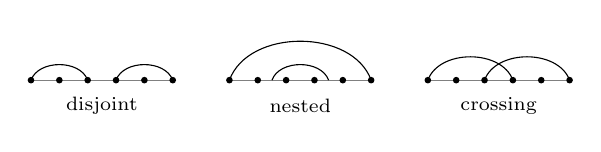
\begin{tikzpicture}[x=0.36cm,y=0.36cm,every node/.style={font=\scriptsize}]
\foreach \o/\lab in {0/disjoint,7/nested,14/crossing}{
  \draw[gray] (\o,0)--(\o+5,0);
  \foreach \x in {0,...,5} \fill (\o+\x,0) circle (1.2pt);
  \node at (\o+2.5,-0.9) {\lab};
}
\draw (0,0) to[out=70,in=110] (2,0);
\draw (3,0) to[out=70,in=110] (5,0);
\draw (7,0) to[out=70,in=110] (12,0);
\draw (8.5,0) to[out=70,in=110] (10.5,0);
\draw (14,0) to[out=70,in=110] (17,0);
\draw (16,0) to[out=70,in=110] (19,0);
\end{tikzpicture}
\caption{The three geometries of a pair of swaps, drawn as arcs over
positions.}
\label{fig:geometry}
\end{figure}

\begin{definition}
$\N_{\mathrm{dyn}}$ contains the moves whose swaps are pairwise
disjoint. $\N_c=\{\sigma:\ncr(\sigma)\leq c\}$, and $\Pa_r$ contains the
moves in which every swap crosses at most $r$ others. $\N_0=\Pa_0$ is
the Motzkin neighborhood and $\N_\infty$ is the set of all involutions.
\end{definition}

``Single crossings'' can mean two things, and we study both: $\N_1$
allows one crossing in the whole move, and $\Pa_1$ allows many crossing
pairs as long as each swap takes part in at most one. The families form
the chains
$\N_{\mathrm{dyn}}\subset\N_0\subset\N_1\subset\N_2\subset\dots\subset\N_\infty$
and $\N_0\subset\N_1\subset\Pa_1\subset\Pa_2\subset\dots\subset\N_\infty$,
with strict inclusions for sufficiently large $n$; $\N_2$ and $\Pa_1$
are incomparable. Figure~\ref{fig:geometry} shows the geometries and
Table~\ref{tab:taxonomy} the sizes.

\begin{table}[t]
\centering
\caption{Size and growth of the neighborhoods on the overlap axis.
Sizes were verified by enumeration for $n\leq 11$.}
\label{tab:taxonomy}
\small
\begin{tabular}{@{}lrrl@{}}
\toprule
Neighborhood & $n=10$ & $n=20$ & Growth \\
\midrule
Dynasearch & 512 & $5.2{\cdot}10^5$ & $2^n$ \\
Motzkin $\N_0$ & 2\,188 & $5.1{\cdot}10^7$ & $3^n n^{-3/2}$ \\
$\N_1$ & 5\,038 & $2.6{\cdot}10^8$ & $M_n\,n/3$ \\
$\N_2$ & 7\,108 & $7.6{\cdot}10^8$ & $M_n\,(n/3)^2/2$ \\
$\Pa_1$ & 5\,263 & $4.9{\cdot}10^8$ & $3.4626^n$ \\
Involutions & 9\,496 & $2.4{\cdot}10^{10}$ & $(n/e)^{n/2}e^{\sqrt n}$ \\
\bottomrule
\end{tabular}
\end{table}

\begin{proposition}\label{prop:jfrac}
Let $I_n(q)=\sum_{\sigma}q^{\ncr(\sigma)}$ over all involutions of $n$
positions and $[h]_q=1+q+\dots+q^{h-1}$. Then
\begin{equation}
\sum_{n\geq0} I_n(q)\,x^n=
\cfrac{1}{1-x-\cfrac{[1]_q\,x^2}{1-x-\cfrac{[2]_q\,x^2}{1-x-\cdots}}}.
\end{equation}
\end{proposition}
\begin{proof}[Sketch]
Read the positions from left to right as a Motzkin path: an opening
endpoint is an up step, a closing endpoint a down step, a fixed point a
level step. A down step from height $h$ may close any of the $h$ open
arcs, and closing the arc that was opened $j$-th from the last creates
$j$ crossings. The weight of the step is therefore $[h]_q$, and
Flajolet's theorem~\cite{flajolet1980} gives the fraction.
\end{proof}

Setting $q=0$ gives the Motzkin numbers $M_n$ and $q=1$ the involution
numbers. The coefficient of $q^c$ counts the moves with exactly $c$
crossings.

\begin{lemma}\label{lem:poisson}
For fixed $c$, the number of involutions of $n$ positions with exactly
$c$ crossings is $M_n\,(n/3)^c/c!\,(1+O(1/n))$. Hence
$|\N_c|\sim M_n(n/3)^c/c!$, and $\N_c$ grows as $3^n$ for every fixed
$c$.
\end{lemma}
\begin{proof}[Sketch]
By Proposition~\ref{prop:jfrac} the coefficient of $q^c$ is a sum over
Motzkin paths of the number of ways to distribute $c$ crossings over the
down steps, where a step from height $h$ carries at most $h-1$. A
typical path has $D\approx n/3$ down steps, of which a bounded number
start at height~1, so the count is
$\mathbb{E}\binom{D+c-1}{c}=(n/3)^c/c!\,(1+O(1/n))$ per path.
\todo{full proof; check whether the statement is known for involutions,
the perfect-matching analogue is Riordan's $\binom{2n}{n-2}$}
\end{proof}

Numerically the ratio of the exact count to the formula for $c=1$ is
$0.82$ at $n=50$ and $0.995$ at $n=2000$. The practical reading is that
a few crossings add little: at $n=50$ the neighborhood $\N_4$ still
covers a fraction $3\cdot10^{-10}$ of all involutions. A uniformly
random involution has about $n^2/24$ crossings, so $\N_c$ for constant
$c$ is the almost-noncrossing corner of the involution set.

\begin{proposition}\label{prop:pa1}
The generating function $S(x)$ of $|\Pa_1|$ satisfies
$S=1+xS+x^2S^2+x^4S^4$, and $|\Pa_1|$ grows as $\rho^{-n}$ with
$\rho^{-1}=3.4626$.
\end{proposition}
\begin{proof}[Sketch]
The first position is a fixed point, the left end of an uncrossed arc,
or the left end of an arc crossed by exactly one other. In the last case
the two arcs have four endpoints, and the three gaps between them and
the remainder after them each hold an independent $\Pa_1$ structure.
\end{proof}

\begin{proposition}\label{prop:optima}
Every family above contains all single swaps. Under additive selection a
permutation is a local optimum of the family if and only if it is a
local optimum of the single-swap neighborhood.
\end{proposition}
\begin{proof}
If no single swap has a negative delta, no sum of deltas is negative.
The converse holds because single swaps are moves of the family.
\end{proof}

Proposition~\ref{prop:optima} sets the overlap axis apart from axes that
bound the reach of a swap. Overlap changes how far a step goes outside
local optima, but it does not change the set of local optima. The
single-swap neighborhood is therefore the natural control for the whole
family.

% ---------------------------------------------------------------------
\section{Exact Move Selection}\label{sec:selection}

For every candidate swap $a=(i,j)$ we compute
$\delta_a=C_{\max}(\pi\circ s(i,j))-C_{\max}(\pi)$ with head and tail
matrices at cost $O(m(j-i))$, which is $O(mn^3)$ for all pairs.
Candidates pass the block-boundary filter of the earlier
studies~\cite{windowed_own}. The predicted change of a compound move is
$\sum_{a\in\sigma}\delta_a$, and selection minimizes it within the
family.

\paragraph{Pruning.} Each family is hereditary: a subset of an
admissible move is admissible. An optimal move therefore uses only
candidates with $\delta_a<0$, and positions that are not an endpoint of
such a candidate can be dropped. Selection runs on the set $C$ of
improving candidates and on their $E\leq 2|C|$ compressed endpoints.

\paragraph{Disjoint and noncrossing moves.} For Dynasearch a positional
program suffices,
$B[p]=\min\bigl(B[p-1],\min_{i<p}B[i-1]+\delta_{ip}\bigr)$. For $\N_0$
let $W[i][j]$ be the best predicted change of a noncrossing move inside
positions $i..j$. Then
\begin{multline}\label{eq:interval}
W[i][j]=\min\Bigl(W[i{+}1][j],\\ \min_{(i,k)\in C,\,k\leq j}
\delta_{ik}+W[i{+}1][k{-}1]+W[k{+}1][j]\Bigr),
\end{multline}
which takes $O(E^2+E|C|)$ time.

\paragraph{Single crossings.} A crossing pair $(i,b),(a,d)$ with
$i<a<b<d$ forms a two-arc core with three inner gaps. For $\Pa_1$ the
recurrence~\eqref{eq:interval} gains one more option at position $i$:
\begin{multline}
\delta_{ib}+\delta_{ad}+W[i{+}1][a{-}1]+W[a{+}1][b{-}1]\\
+W[b{+}1][d{-}1]+W[d{+}1][j],
\end{multline}
minimized over the cores that start at $i$ and end by $j$. No arc inside
a gap can cross a core arc, because the core arcs are already crossed
once. For $\N_1$ the program keeps two tables, one for noncrossing moves
and one for moves with exactly one core, and a core is closed with
noncrossing gaps. The cores are enumerated from pairs of crossing
candidates in $O(|C|^2)$ and the tables are filled in $O(E^3)$. For
$c\geq2$ the connected components of the crossing graph have at most
$c+1$ arcs, which gives cores of bounded size and a knapsack over the
crossing budget. \todo{Algorithm~1: the $\Pa_1$ program as pseudocode;
state the $c=2$ program or leave it to an appendix}

\paragraph{Involutions.} Without a crossing constraint the candidates
are the edges of a graph on the positions with weights $-\delta_a$, and
the best move is a maximum-weight matching~\cite{edmonds1965}, found in
$O(n^3)$.

\paragraph{Cost.} \todo{E0 on the campaign machine.} In the pilot the
selection on states taken from a search trajectory took at most
$0.6$\,ms for $\N_0$, $4.5$\,ms for $\N_1$ and $\Pa_1$ and $1.3$\,ms for
involutions, against $14$--$221$\,ms for the deltas at $n=50$--$100$.
Dense states are the exception. Right after the start, or after a move
that made the schedule much worse, thousands of candidates improve, and
the core enumeration becomes the bottleneck. We therefore restrict the
cores to the $400$ most improving candidates and the matching to the
$3000$ most improving ones, and we record how often a cap is active.

\paragraph{Acceptance.} The selected move is applied as it is; when no
candidate improves, the best single swap is applied. This is the rule of
the earlier Dynasearch and Motzkin implementations, and every result in
the main study uses it. Section~\ref{sec:safe} treats a variant that
checks the real makespan before applying the move.

% ---------------------------------------------------------------------
\section{Additivity by Pair Geometry}\label{sec:additivity}

The selection optimizes a sum of deltas, but the makespan change of two
swaps is not the sum of their changes. In the lattice-path view the
makespan is the length of a longest path through the grid of operations,
$C'_{\max}=\max_P\bigl[\ell(P)+\sum_a\Delta_a(P)\bigr]$. Two disjoint
swaps interact only through the choice of the critical path. A nested or
crossing pair also changes the jobs that lie inside each other's
interval, so each delta is computed in a context that the other swap
destroys. We write the second-order term as
$Q_{ab}=\Delta_{ab}-\delta_a-\delta_b$, where $\Delta_{ab}$ is the real
change of the pair. \todo{minimal counterexamples for each geometry and
a sufficient condition for $Q_{ab}=0$}

\begin{table}[t]
\centering
\caption{PILOT: realized share of the predicted joint gain of two
improving swaps on trajectory states; in parentheses the share of pairs
that do not improve together.}
\label{tab:geometry}
\small
\begin{tabular}{@{}rccc@{}}
\toprule
$n$ & disjoint & nested & crossing \\
\midrule
20 & 0.66 (7\%) & 0.30 (32\%) & 0.37 (27\%) \\
50 & 0.61 (11\%) & 0.34 (25\%) & 0.23 (31\%) \\
100 & 0.52 (12\%) & 0.22 (27\%) & 0.12 (34\%) \\
\bottomrule
\end{tabular}
\end{table}

Table~\ref{tab:geometry} reports the pilot measurement. Disjoint pairs
realize more than half of their predicted gain, and overlapping pairs
realize between a tenth and a third. Nested and crossing pairs do not
differ consistently: at $n=20$ nested pairs are worse, at $n\geq50$
crossing pairs are. Overlap breaks additivity, and crossing as such does
not. On start states all three geometries are close to additive, so the
effect belongs to the region near local optima where the search spends
its time.

The consequence for whole moves is that the families trade predicted
gain for realized gain. On trajectory states the noncrossing optimum
already holds most of the predicted gain of the involution optimum, and
Dynasearch holds the least. Dynasearch, however, realizes a positive
share of its prediction, whereas the moves selected from $\N_0$ and from
the involutions make the makespan worse on average at $n\geq50$. The
best involution also has many crossings, from a handful at $n=20$ to
tens at $n=50$, so a small crossing budget does not reproduce it.
\todo{E1: figure of predicted and realized gain along the axis, figure
of additivity by geometry, histogram of crossings in the involution
optimum; replace the pilot numbers}

% ---------------------------------------------------------------------
\section{Experiments}\label{sec:exp}

The protocol is that of the earlier studies~\cite{windowed_own}, and the
neighborhood family is the only factor. The
instances are the 120 Taillard instances~\cite{taillard1993} in 12
classes with $n\in\{20,50,100,200,500\}$ and $m\in\{5,10,20\}$. The
metaheuristic is the unchanged ILS with a tabu list of tenure 10 and an
elite pool of the 10 best solutions perturbed by double-bridge kicks,
started from the identity permutation. Each configuration runs once for
$10$\,s per seed with 5 seeds, and the incumbents at $0.1$, $0.5$, $1$,
$2$ and $5$\,s are read from the trajectory log, which is valid because
the time limit acts only as a stopping rule. The variants are
Dynasearch, $\N_0$, $\N_1$, $\Pa_1$ and involutions, with the best
single swap as a control. All
variants share one implementation of candidates, deltas and filter. Runs
are sequential on an Apple M4 Pro.

Quality is the relative percentage deviation (RPD) from the Taillard
lower bound at $10$\,s. Conclusions are drawn only in classes where a
$10$\,s run makes at least 30 moves, which we expect for $n\leq100$ (nine
classes); at $n=500$ a run makes a single move. Two families of tests
were fixed before the campaign, each with instances as blocks and Holm
correction over the classes: involutions against $\N_0$, and Dynasearch
against $\N_0$, two-sided. Page's trend test~\cite{page1963} is applied
along the chain
$\N_{\mathrm{dyn}}\subset\N_0\subset\N_1\subset\Pa_1\subset\N_\infty$.
All other comparisons are exploratory and reported as such. Families
with crossings complete fewer iterations, so the first family is also
analyzed at equal iteration counts.

\begin{table}[t]
\centering
\caption{PILOT: mean RPD [\%] to the lower bound, ILS, 4 instances
$\times$ 3 seeds per class, Apple M4 Pro.}
\label{tab:pilot}
\small
\begin{tabular}{@{}lccc@{}}
\toprule
 & $20\times5$ & $20\times10$ & $50\times10$ \\
Variant & 1\,s / 5\,s & 1\,s / 5\,s & 1\,s / 5\,s \\
\midrule
Single swap & 3.68 / 3.18 & 9.53 / 9.00 & 6.88 / 5.91 \\
Dynasearch & 3.49 / 3.08 & 9.32 / 8.84 & 6.24 / 4.93 \\
$\N_0$ (Motzkin) & 3.41 / 3.10 & 9.42 / 8.76 & 17.84 / 13.69 \\
$\N_1$ & 3.75 / 3.21 & 9.86 / 9.32 & 17.81 / 16.18 \\
$\Pa_1$ & 3.75 / 3.27 & 10.17 / 9.41 & 19.27 / 16.89 \\
Involutions & 6.44 / 4.41 & 16.95 / 12.91 & 24.16 / 22.82 \\
\bottomrule
\end{tabular}
\end{table}

\begin{table*}[t]
\centering
\caption{SKELETON: mean RPD [\%] to the lower bound at $10$\,s, ILS, per
class (10 instances, 5 seeds).}
\label{tab:main}
\small
\begin{tabular}{@{}l*{12}{c}@{}}
\toprule
Variant & \multicolumn{3}{c}{$n=20$} & \multicolumn{3}{c}{$n=50$} &
\multicolumn{3}{c}{$n=100$} & \multicolumn{2}{c}{$n=200$} & $n=500$ \\
$m$ & 5 & 10 & 20 & 5 & 10 & 20 & 5 & 10 & 20 & 10 & 20 & 20 \\
\midrule
Single swap & -- & -- & -- & -- & -- & -- & -- & -- & -- & -- & -- & -- \\
Dynasearch & -- & -- & -- & -- & -- & -- & -- & -- & -- & -- & -- & -- \\
$\N_0$ (Motzkin) & -- & -- & -- & -- & -- & -- & -- & -- & -- & -- & -- & -- \\
$\N_1$ & -- & -- & -- & -- & -- & -- & -- & -- & -- & -- & -- & -- \\
$\Pa_1$ & -- & -- & -- & -- & -- & -- & -- & -- & -- & -- & -- & -- \\
Involutions & -- & -- & -- & -- & -- & -- & -- & -- & -- & -- & -- & -- \\
\bottomrule
\end{tabular}
\end{table*}

\paragraph{Pilot.} Table~\ref{tab:pilot} shows the pilot. Its patterns
are hypotheses until the campaign confirms them, and the pilot evaluated
all pairs without the block filter. Quality falls along the axis.
Involutions are worse than $\N_0$ in every instance of every class at
both budgets, and at $50\times10$ the families with crossings are worse
than $\N_0$ at $5$\,s, while at $1$\,s $\N_1$ and $\N_0$ are level.
Dynasearch is the best family at $50\times10$, far ahead of $\N_0$. At
$n=20$ Dynasearch and $\N_0$ are within a tenth of a point of each
other, $\N_1$ and $\Pa_1$ trail them by up to $0.8$ points, and the
involutions fall far behind. The best compound family gains $0.6$--$1.0$
points over the single swap at $n=50$ and at most $0.3$ at $n=20$.

These patterns fit the measurement of Section~\ref{sec:additivity}. ILS
with a tabu list applies the selected move even when it makes the
schedule worse. For disjoint swaps such a move is mildly worse; for
overlapping swaps it is often much worse. The same mechanism accounts
for the weak Motzkin results at $n\geq50$ in the earlier scaling
study~\cite{windowed_own}, which used the same rule.
\todo{wording agreed with the supervisor}
\todo{replace with the campaign: Table~\ref{tab:main}, figure of RPD
along the axis, iterations per budget, ablations (exact critical-path
filter, cap on the candidates); in the anatomy, the share of states in
which the selected move is worse than the best single swap}

% ---------------------------------------------------------------------
\section{A Safeguarded Variant}\label{sec:safe}

The pilot raises an obvious question: how much of the loss comes from
moves that the search would reject if it looked at their real makespan?
To answer it we run a separate variant. The makespan of the selected
compound move is evaluated once, at cost $O(mn)$, and the better of this
move and the best single swap is applied, so a step is never worse than
the best single swap. This changes the selection rule and not the
neighborhood, so the variant stays out of the main tables and out of the
pre-registered tests, and it is not comparable with the earlier
Dynasearch and Motzkin results.

\begin{table}[t]
\centering
\caption{PILOT, safeguarded variant: mean RPD [\%] to the lower bound,
same runs as Table~\ref{tab:pilot}.}
\label{tab:safe}
\small
\begin{tabular}{@{}lccc@{}}
\toprule
 & $20\times5$ & $20\times10$ & $50\times10$ \\
Variant & 1\,s / 5\,s & 1\,s / 5\,s & 1\,s / 5\,s \\
\midrule
Dynasearch & 3.51 / 3.21 & 9.41 / 8.92 & 7.00 / 5.52 \\
$\N_0$ (Motzkin) & 3.23 / 2.96 & 9.43 / 9.06 & 5.99 / 5.17 \\
$\N_1$ & 3.16 / 2.96 & 9.33 / 8.86 & 6.30 / 5.34 \\
$\Pa_1$ & 3.21 / 2.98 & 9.16 / 8.80 & 6.72 / 5.53 \\
Involutions & 3.07 / 2.95 & 9.56 / 8.79 & 6.16 / 5.55 \\
\bottomrule
\end{tabular}
\end{table}

Table~\ref{tab:safe} shows that the check removes most of the loss of
the overlapping families. At $50\times10$ it brings $\N_0$ from $17.84$
to $5.99$ and the involutions from $24.16$ to $6.16$ at $1$\,s, and the
four overlapping families then differ by less than one point. Dynasearch, in contrast, gets worse
with the check. The safeguarded overlapping families end up close to
Dynasearch without the check: at $1$\,s safeguarded $\N_0$ is slightly
ahead of it, at $5$\,s Dynasearch is ahead of all of them. A cheap check of the real makespan thus matters more than the
choice among overlapping families. \todo{replace with the campaign stage
with the safeguard}

% ---------------------------------------------------------------------
\section{QUBO Structure}\label{sec:quantum}

As a QUBO over the candidate swaps, a family is a set of penalties on
pairs of candidates. The Motzkin QUBO penalizes pairs that share an
endpoint and pairs that cross. The involution QUBO penalizes only shared
endpoints. The largest neighborhood on the axis therefore has the
sparsest QUBO. A third model adds the measured terms $Q_{ab}$ and
expresses what no interval program can; it is the densest.

\begin{table}[t]
\centering
\caption{PILOT: couplers and physical qubits on a Pegasus graph for the
Motzkin (M), involution (I) and pair-corrected (PQ) QUBO over the same
$K$ candidates.}
\label{tab:qubo}
\small
\begin{tabular}{@{}lrcc@{}}
\toprule
State & $K$ & Couplers M / I / PQ & Qubits M / I / PQ \\
\midrule
$20\times10$ & 18 & 59 / 41 / 140 & 26 / 22 / 45 \\
$20\times20$ & 11 & 27 / 13 / 55 & 14 / 10 / 20 \\
$50\times10$ & 105 & 2117 / 634 / -- & 1001 / 425 / -- \\
\bottomrule
\end{tabular}
\end{table}

Table~\ref{tab:qubo} shows the structure on three trajectory states. We
plan to use the processor as an oracle on stored states: for each state
the three QUBOs over the same candidates are sampled and compared with
the exact optimum. Two end points are kept apart. Hardware fidelity is
the energy gap to the optimum of the sampled model and the share of
feasible samples. Move quality is the real makespan change. The
involution QUBO may win the first and lose the second, because its
optimum contains more overlapping swaps. \todo{E4: annealer and
gate-based results, or cut the section to one paragraph}

% ---------------------------------------------------------------------
\section{Conclusions}
\todo{depends on the campaign. Pilot reading: under additive
selection swaps should not cross, and in this protocol not even nest;
disjoint moves predict less and deliver more. With a makespan check the
overlapping families recover, but they do not beat Dynasearch.
Crossings could pay off only with a model of pair interactions, which a
QUBO can express and a dynamic program cannot.}

% ---------------------------------------------------------------------
% All entries to be verified in Crossref (authors, volume, pages, DOI).
\begin{thebibliography}{99}\small
\bibitem{ahuja2002} R.K.~Ahuja, \"O.~Ergun, J.B.~Orlin, A.P.~Punnen.
A survey of very large-scale neighborhood search techniques.
\emph{Discrete Appl.\ Math.} 123:75--102, 2002.
\bibitem{akutsu2000} T.~Akutsu. Dynamic programming algorithms for RNA
secondary structure prediction with pseudoknots. \emph{Discrete Appl.\
Math.} 104:45--62, 2000. \todo{verify}
\bibitem{bozejko2007} W.~Bo\.zejko, M.~Wodecki. On the theoretical
properties of swap multimoves. \emph{Oper.\ Res.\ Lett.} 35(2):227--231, 2007.
\bibitem{bozejko2026sr} W.~Bo\.zejko, M.~Uchro\'nski, M.~Wodecki. The new
exponential Fibonacci neighborhood as QUBO generated on a D-Wave quantum
computing environment for the permutational scheduling problem.
\emph{Sci.\ Rep.}, 2026.
\bibitem{chen2007} W.Y.C.~Chen, E.Y.P.~Deng, R.R.X.~Du, R.P.~Stanley,
C.H.~Yan. Crossings and nestings of matchings and partitions.
\emph{Trans.\ Amer.\ Math.\ Soc.} 359:1555--1575, 2007. \todo{verify}
\bibitem{congram2002} R.K.~Congram, C.N.~Potts, S.L.~van de Velde. An
iterated dynasearch algorithm for the single-machine total weighted
tardiness scheduling problem. \emph{INFORMS J.\ Comput.} 14(1):52--67, 2002.
\bibitem{deineko2000} V.G.~Deineko, G.J.~Woeginger. A study of
exponential neighborhoods for the travelling salesman problem and for
the quadratic assignment problem. \emph{Math.\ Program.} 87:519--542,
2000. \todo{verify}
\bibitem{edmonds1965} J.~Edmonds. Paths, trees, and flowers.
\emph{Canad.\ J.\ Math.} 17:449--467, 1965.
\bibitem{ergun2006} \"O.~Ergun, J.B.~Orlin. Fast neighborhood search for
the single machine total weighted tardiness problem. \emph{Oper.\ Res.\
Lett.} 34(1):41--45, 2006. \todo{verify}
\bibitem{fibonacci_own} \todo{own work, third person: Fibonacci neighborhood}
\bibitem{flajolet1980} P.~Flajolet. Combinatorial aspects of continued
fractions. \emph{Discrete Math.} 32(2):125--161, 1980.
\bibitem{garey1976} M.R.~Garey, D.S.~Johnson, R.~Sethi. The complexity of
flowshop and jobshop scheduling. \emph{Math.\ Oper.\ Res.} 1(2):117--129, 1976.
\bibitem{grosso2004} A.~Grosso, F.~Della Croce, R.~Tadei. An enhanced
dynasearch neighborhood for the single-machine total weighted tardiness
scheduling problem. \emph{Oper.\ Res.\ Lett.} 32(1):68--72, 2004. \todo{verify}
\bibitem{gutin1999} G.~Gutin. Exponential neighbourhood local search for
the traveling salesman problem. \emph{Comput.\ Oper.\ Res.}
26:313--320, 1999. \todo{verify}
\bibitem{kasraoui2006} A.~Kasraoui, J.~Zeng. Distribution of crossings,
nestings and alignments of two edges in matchings and partitions.
\emph{Electron.\ J.\ Combin.} 13, R33, 2006. \todo{verify}
\bibitem{lyngso2000} R.B.~Lyngs\o, C.N.S.~Pedersen. RNA pseudoknot
prediction in energy-based models. \emph{J.\ Comput.\ Biol.}
7(3--4):409--427, 2000. \todo{verify}
\bibitem{motzkin_own} \todo{own work, third person: Motzkin neighborhood}
\bibitem{nussinov1978} R.~Nussinov, G.~Pieczenik, J.R.~Griggs,
D.J.~Kleitman. Algorithms for loop matchings. \emph{SIAM J.\ Appl.\
Math.} 35(1):68--82, 1978.
\bibitem{page1963} E.B.~Page. Ordered hypotheses for multiple
treatments: a significance test for linear ranks. \emph{J.\ Amer.\
Statist.\ Assoc.} 58:216--230, 1963.
\bibitem{riordan1975} J.~Riordan. The distribution of crossings of
chords joining pairs of $2n$ points on a circle. \emph{Math.\ Comp.}
29:215--222, 1975.
\bibitem{rivas1999} E.~Rivas, S.R.~Eddy. A dynamic programming algorithm
for RNA structure prediction including pseudoknots. \emph{J.\ Mol.\
Biol.} 285(5):2053--2068, 1999.
\bibitem{ruiz2007} R.~Ruiz, T.~St\"utzle. A simple and effective iterated
greedy algorithm for the permutation flowshop scheduling problem.
\emph{Eur.\ J.\ Oper.\ Res.} 177(3):2033--2049, 2007.
\bibitem{sarvanov1981} V.I.~Sarvanov, N.N.~Doroshko. Approximate
solution of the travelling salesman problem by a local algorithm that
searches neighbourhoods of factorial cardinality in cubic time.
1981. \todo{verify source}
\bibitem{schuirmann1987} D.J.~Schuirmann. A comparison of the two
one-sided tests procedure and the power approach for assessing the
equivalence of average bioavailability. \emph{J.\ Pharmacokinet.\
Biopharm.} 15:657--680, 1987.
\bibitem{tabaska1998} J.E.~Tabaska, R.B.~Cary, H.N.~Gabow, G.D.~Stormo.
An RNA folding method capable of identifying pseudoknots and base
triples. \emph{Bioinformatics} 14(8):691--699, 1998.
\bibitem{taillard1993} E.~Taillard. Benchmarks for basic scheduling
problems. \emph{Eur.\ J.\ Oper.\ Res.} 64(2):278--285, 1993.
\bibitem{touchard1952} J.~Touchard. Sur un probl\`eme de configurations
et sur les fractions continues. \emph{Canad.\ J.\ Math.} 4:2--25, 1952.
\bibitem{windowed_own} \todo{own work, third person: windowed QUBO / classical--quantum neighborhoods}
\end{thebibliography}
\end{document}
